\section{Non local Maxwell Condition}

{\color{red}Traveling pulses are a generic feature of spatially-extended excitable systems (Idema et al., 2013, Ryan et al., 2012, Bement et al., 2015). In many cases, neighboring regions are coupled by the diffusion of a molecular participant. In these reaction-diffusion systems, a simple mathematical condition exists for determining whether an excitation will induce a traveling pulse or remain localized, sometimes called the Maxwell condition (Britton, 1982, Mori et al., 2008). Since our system is not a reaction-diffusion system, the Maxwell condition fails to predict whether the blebs travel or not. }

We seek an analog of the Maxwell condition for the bleb model, and similar non-local PDEs. In the fast timescale, we have $c = c^{ss}$.  The dynamics of excitation are thus only governed by the $a$ equation. We will make progress on this by studying the following systems, from most general to most narrow.
\begin{enumerate}[label=(\Alph*)]
\item \textbf{Ultimately, we are interested in a necessary and sufficient traveling wave condition for the general}
\begin{align}
\dfrac{\partial a}{ \partial t}  & =  f(a,y)\\
0 & =g \left(a,y,\dfrac{\partial^2 y}{\partial x^2}\right).
\end{align}
We have not yet succeeded in this. 
\item\textbf{The specific system we are interested in is}
\begin{align}
\dfrac{\partial a}{ \partial t}  & =  \dfrac{c^{ss}}{1+c^{ss}} \mbox{exp}\left(-\dfrac{y-y_C}{D}\right) - a \mbox{exp} \left(\dfrac{y-y_C}{F} \right)\label{eq::a_ODE}\\
0 & = -a(y - y_C) + P (1-y) + \gamma_M \dfrac{\partial^2 y}{\partial x^2}\label{eq::yM_eq} \\
0 & = a(y-y_C) - Mcy_C\label{eq::nondimyC2}.
\end{align} 
Note that since Eq.~\ref{eq::nondimyC2} is algebraic in $y_C$, we can eliminate it from the system, and (B) is indeed a special case of (A). 
\item \textbf{A narrow version of the system is obtained if we assume the force balance equations are linear in $a$}
\begin{align}
\dfrac{da}{ dt}  & = f_1(y) - a f_2(y)\label{eq::gen_a}\\
0 & = g_1(y) - ag_2(y) +  \dfrac{\partial^2 y}{\partial x^2}\label{eq::gen_ym}
\end{align}
\item \textbf{This can be obtained from our system given the following simplifying assumption.} Assume that the cortex does not move significantly during excitation, $y_C = y_C^{ss}$, leaving us with the new system of two equations:
\begin{align}
\dfrac{\partial a}{ \partial t}  & =  \dfrac{c^{ss}}{1+c^{ss}} \mbox{exp}\left(-\dfrac{y-y_C^{ss}}{D}\right) - a \mbox{exp} \left(\dfrac{y-y_C^{ss}}{F} \right)\label{eq::a_ODE}\\
0 & = -a(y - y_C^{ss}) + P (1-y) + \gamma_M \dfrac{\partial^2 y}{\partial x^2}\label{eq::yM_eq}
\end{align} 
\end{enumerate}
We derive a necessary condition for this system (C) here. A travelling wave solution to this system is shown in Fig.~\ref{fig::A_wave}.
\begin{figure}[h]
\centering
\captionsetup{width=.9\linewidth}
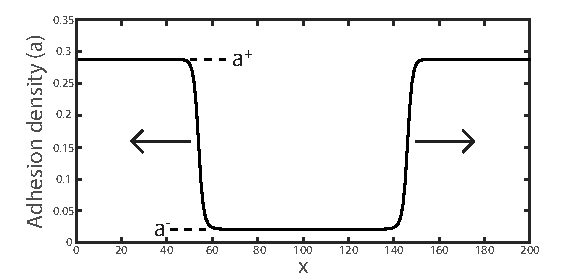
\includegraphics[width=4.5in]{Project2/figs/A_wave.pdf}
\caption{Snapshot of the travelling wave from simulation of Eq.~\ref{eq::a_ODE} and~\ref{eq::yM_eq}.}
\label{fig::A_wave}
\end{figure}

We assume, WLOG, that Eq.~\ref{eq::gen_a} has two stable roots which we will denote by $(y^{+},a^{+})$ and $ (y^{-},a^{-})$.
Transform to wave coordinate $z = x-vt$ and~\ref{eq::gen_a} and~\ref{eq::gen_ym} become:
\begin{align}
-v \dfrac{da}{ dz}  & = f_1(y) - a f_2(y)\label{eq::gen_a_z}\\
0 & = g_1(y) - ag_2(y) +  \dfrac{\partial^2 y}{\partial z^2}\label{eq::gen_ym_z}
\end{align}
We can use Eq.~\ref{eq::gen_ym_z} to solve for $a$:
\begin{flalign}
 a = \dfrac{1}{g_2(y)} \left( g_1(y) + \dfrac{\partial^2 y}{\partial z^2} \right)
\end{flalign}
Then it follows that:
\begin{equation}\Rightarrow  -v \dfrac{\partial a}{ \partial z}   =  f_1(y)  -  \dfrac{g_1(y)}{g_2(y)}f_2(y) - \dfrac{f_2(y)}{g_2(y)} \dfrac{\partial^2 y}{\partial z^2}
\end{equation}
Multiply by $ \dfrac{g_2(y)}{f_2(y)} $,
\begin{equation}\Rightarrow   -v \dfrac{\partial a}{ \partial z} \dfrac{g_2(y)}{f_2(y)}   =  f_1(y)\dfrac{g_2(y)}{f_2(y)}  -  g_1(y) -  \dfrac{\partial^2 y}{\partial z^2}
\end{equation}
Multiply by $\dfrac{\partial y}{\partial z}$,
\begin{equation}\Rightarrow  -v \dfrac{\partial a}{ \partial z} \dfrac{g_2(y)}{f_2(y)} \dfrac{\partial y}{\partial z}   =  \left( f_1(y)\dfrac{g_2(y)}{f_2(y)}  -  g_1(y) -  \dfrac{\partial^2 y}{\partial z^2} \right)  \dfrac{\partial y}{\partial z}
\end{equation}
Integrate over $z$, 
\begin{equation}
\Rightarrow  \int_ {- \infty}^{\infty}  -v \dfrac{\partial a}{ \partial z} \dfrac{g_2(y)}{f_2(y)} \dfrac{\partial y}{\partial z} dz = \int_ {- \infty}^{\infty} \left( f_1(y)\dfrac{g_2(y)}{f_2(y)}  -  g_1(y) -  \dfrac{\partial^2 y}{\partial z^2} \right)  \dfrac{\partial y}{\partial z} dz
\end{equation}
Change variables on RHS,   
\begin{align}\Rightarrow -v  \int_ {- \infty}^{\infty}  \dfrac{\partial a}{ \partial z} \dfrac{g_2(y)}{f_2(y)} \dfrac{\partial y}{\partial z} dz &= \int_ {y^{-}}^{y^{+}} \left( f_1(y)\dfrac{g_2(y)}{f_2(y)}  -  g_1(y) -  \dfrac{\partial^2 y}{\partial z^2} \right)  dy \\
\Rightarrow  -v  \int_ {- \infty}^{\infty}  \dfrac{\partial a}{ \partial z} \dfrac{g_2(y)}{f_2(y)} \dfrac{\partial y}{\partial z} dz &= \int_ {y^{-}}^{y^{+}} \left( f_1(y)\dfrac{g_2(y)}{f_2(y)}  -  g_1(y)\right) dy -  \cancelto{0}{\int_ {y^{-}}^{y^{+}}  \dfrac{\partial^2 y}{\partial z^2}   dy}\\
\Rightarrow -v  \int_ {- \infty}^{\infty}  \dfrac{\partial a}{ \partial z} \dfrac{g_2(y)}{f_2(y)} \dfrac{\partial y}{\partial z} dz &= \int_ {y^{-}}^{y^{+}} \left( f_1(y)\dfrac{g_2(y)}{f_2(y)}  -  g_1(y)\right) dy 
\end{align}
The Non-local Maxwell Condition Number is defined by the RHS of the above equation. In our specific case,
\begin{align}
f_1(y) &=  \dfrac{c^{ss}}{1+c^{ss}} \mbox{exp}\left(-\dfrac{y-y_C^{ss}}{D}\right),\\
f_2(y) &= \mbox{exp} \left(\dfrac{y-y_C^{ss}}{F} \right),\\
g_1(y) &=  P (1-y), \\
 g_2(y) &= (y - y_C^{ss}).
\end{align}
Therefore, 
\begin{multline}
-v  \int_ {- \infty}^{\infty}  \dfrac{\partial a}{ \partial z} \dfrac{(y - y_C^{ss})}{ \mbox{exp} \left(\dfrac{y-y_C^{ss}}{F} \right)} \dfrac{\partial y}{\partial z} dz \\
= \int_ {y^{-}}^{y^{+}} \left( \dfrac{c^{ss}}{1+c^{ss}} \mbox{exp}\left(-\dfrac{y-y_C^{ss}}{D}\right) \dfrac{(y - y_C^{ss})}{ \mbox{exp} \left(\dfrac{y-y_C^{ss}}{F} \right)}  -   P (1-y) \right) dy
\end{multline}
\begin{multline}
\implies -v  \int_ {- \infty}^{\infty}  \dfrac{\partial a}{ \partial z}\dfrac{\partial y}{\partial z} \mbox{exp} \left(-\dfrac{y-y_C^{ss}}{F} \right)(y - y_C^{ss}) dz\\
= \int_ {y^{-}}^{y^{+}}  \left( \dfrac{c^{ss}}{1+c^{ss}} \mbox{exp}\left( -\left( \dfrac{1}{D} + \dfrac{1}{F} \right) (y-y_C^{ss})\right)  -   P (1-y) \right) dy\\
\end{multline}
We also note that in our specific case $y^- > y^+$ and so it makes sense to integrate from $y^+$ to $ y^-$.
\begin{align*}
\Rightarrow & -v  \int_ {- \infty}^{\infty}  \dfrac{\partial a}{ \partial z}\dfrac{\partial y}{\partial z} \mbox{exp} \left(-\dfrac{y-y_C^{ss}}{F} \right)(y - y_C^{ss}) dz\\
& \hspace{2cm}= - \int_ {y^{+}}^{y^{-}}  \left( \dfrac{c^{ss}}{1+c^{ss}} \mbox{exp}\left( -\left( \dfrac{1}{D} + \dfrac{1}{F} \right) (y-y_C^{ss})\right)  -   P (1-y) \right) dy
\end{align*}
Our Non-Local Maxwell condition Number is:
\begin{align}
NLMC &= -\int_ {y^{+}}^{y^{-}}  \left( \dfrac{c^{ss}}{1+c^{ss}} \mbox{exp}\left( -\left( \dfrac{1}{D} + \dfrac{1}{F} \right) (y-y_C^{ss})\right)  -   P (1-y) \right) dy \\
 &= \dfrac{c^{ss}}{1+c^{ss}}  \mbox{exp}\left( +\left( \dfrac{1}{D} + \dfrac{1}{F} \right)y_C^{ss}  \right) \left( y^--y^+ \right) + P\left( 1 - \frac{1}{2}\left( \left(y^+\right)^2-\left(y^-\right)^2\right)\right)
\end{align}
The integral on the LHS is of determined sign (-).  Therefore, the Nonlocal Maxwell Condition is:
\begin{align*}
& NLMC >0 \Rightarrow v \text{ exists, travelling solution}\\
& NLMC <0 \Rightarrow v \text{ does not exist, stationary solution}
\end{align*}
Note that only the second line (necessity) is shown here. The first line (sufficiency) is supported by numerical evidence below.

